This section is devoted to a specific description of every kind of requirement the system has to deal with in order to achieve all the functionalities described.


\section{External interface requirements}
\label{sec:external_interface_requirements}%

\subsection{User interfaces}
\label{subsec:User_interfaces}%
The CodeKataBattle’s User interface will be a website, developed in order to be used both by STs and EDs, available to everybody who has a device with an Internet Browser and a reliable Internet connection.

\subsection{Hardware interfaces}
\label{subsec:hardware_interfaces}%
The system will be accessible from every device with an Internet Browser to access the website and a reliable Internet connection.\\
The User is free to choose his device like a computer, a tablet or a smartphone, despite that, it is suggested to use a computer, which will make it easier to deal with the writing of the code.

\subsection{Software interfaces}
\label{subsec:software_interfaces}%
The system requires the GitHub APIs and the External Tools in order to work properly. Also, it will use a mailing system to send confirmation eMails to the Users during the registration process.    

\subsection{Communication interfaces}
\label{subsec:communication_interfaces}%
The communication Interfaces needed by the system are the HTTPS Protocol and the Mail System Transfer Protocol (SMTP).

\section{Functional requirements}
\label{sec:functional_requirements}%

\subsection{Requirements}
\label{subsec:requirements3}%
\newcounter{req}
\setcounter{req}{1}
\newcommand{\creq}{\thereq\stepcounter{req}}
\begin{center}
    \begin{longtable}{|l|p{0.9\linewidth}|}
        \hline
        \textbf{ID} & \textbf{Description}                                                                                                                             \\
        \hline
        R\creq      & CKB allows unregistered Users to sign up                                                                    \\
        \hline
        R\creq      & CKB allows registered EDs to login                                                                    \\
        \hline
        R\creq      & CKB allows registered STs to login                                                                    \\
        \hline
        R\creq      & CKB allows EDs to create Tournaments                                                                    \\
        \hline
        R\creq      & CKB allows EDs to grant the permissions of a Tournament to other EDs                                                                 \\
        \hline
        R\creq      & CKB allows EDs to create Battles                                                                    \\
        \hline
        R\creq      & CKB allows EDs to uploads the code kata of a Battle                                                                   \\
        \hline
        R\creq      & CKB allows EDs to set the minimum and the maximum number of STs per group of a Battle                                                            \\
        \hline
        R\creq      & CKB allows EDs to set a registration deadline of a Battle                                                                 \\
        \hline
        R\creq      & CKB allows EDs to set a submission deadline of a Battle                                                                \\
        \hline
        R\creq      & CKB allows EDs to set additional configuration for the scoring system of a Battle                                                                \\
        \hline
        R\creq      & CKB allows EDs to set functional aspects for the scoring system of a Battle                                                               \\
        \hline
        R\creq      & CKB allows EDs to create new Badges                                                  \\
        \hline
        R\creq      & CKB allows EDs to choose the rules related to the awarding of Badges                                                               \\
        \hline
        R\creq      & CKB allows EDs to choose which Badges to award in a certain Tournament                                                               \\
        \hline
        R\creq      & CKB allows EDs to assign a score manually during the consolidation stage                                                               \\
        \hline
        R\creq      & CKB allows EDs to close a Tournament                                                               \\
        \hline
        R\creq      & CKB allows EDs to visualize the profile of another User                                                               \\
        \hline
        R\creq      & CKB allows STs to visualize the profile of another User \\
        \hline
        R\creq      & CKB allows STs to join a Tournament \\
        \hline
        R\creq      & CKB allows STs to join a Battle \\
        \hline
        R\creq      & CKB allows STs to create a new STG \\
        \hline
        R\creq      & CKB allows STs to join a STG \\
        \hline
        R\creq      & CKB allows STs to invite other STs in their STG \\
        \hline
        R\creq      & CKB stores the informations about the Users \\
        \hline
        R\creq      & CKB shall ensure security of data \\
        \hline
        R\creq      & CKB sends notifications to every ST when a new Tournament is created \\
        \hline
        R\creq      & CKB sends notifications when a new Battle is created to every ST which is participating in the Tournament that the Battle is part of \\
        \hline
        R\creq      & CKB sends notifications to a ST when he receives an invitation to be part of STG \\
        \hline
        R\creq      & CKB creates a GH repository of the code kata when the registration deadline for the Battle expires \\
        \hline
        R\creq      & CKB sends the link of the GH repository to every STG that participates in the Battle \\
        \hline
        R\creq      & CKB evaluates the STG's work every time a push is made on GH and calculates Battle score for the STG \\
        \hline
        R\creq      & CKB updates the Battle Leaderboard once a new score is registered \\
        \hline
        R\creq      & CKB updates the Tournament Leaderboard once a new score is registered \\
        \hline
        R\creq      & CKB allows STs to check the Leaderboard of a Battle \\
        \hline
        R\creq      & CKB allows EDs to check the Leaderboard of a Battle \\
        \hline
        R\creq      & CKB allows EDs to analyze the code of a STG \\
        \hline
        R\creq      & CKB sends notifications to every STs participating in the Battle once the consolidation stage ends \\
        \hline
        R\creq      & CKB allows STs to check the list of ongoing Tournaments \\
        \hline
        R\creq      & CKB allows EDs to check the list of ongoing Tournaments \\
        \hline
        R\creq      & CKB allows STs to check the Leaderboard of a Tournament \\
        \hline
        R\creq      & CKB allows EDs to check the Leaderboard of a Tournament \\
        \hline
        R\creq      & CKB sends notification to every ST involved in a Tournament when the Tournament is closed and the final ranks are available \\
        \hline
        R\creq      & CKB shall communicate with the GH API in order to calculate a new score every time a push action is made by a STG \\
        \hline
        R\creq      & CKB shall communicate with the external tool in order to calculate the score of a STG \\
        \hline
        R\creq      & CKB shall communicate with the mailing system in order to allow Users to register their account\\
        \hline
        R\creq      & STs need to fork the GH repository of the Battle they are participating in \\
        \hline
        R\creq      & STs need to push their code in the GH repository in order to have their code evaluated\\
        \hline
        R\creq      & CKB shall assign the Badges to all STs that fullfill their requirements \\
        \hline
        R\creq      & CKB sends notifications to the ED when he receives the permission to create Battles in a Tournament\\
        \hline
        \caption{Requirements.}
        \label{tab: req}%
    \end{longtable}
\end{center}

\subsection{Use case diagrams}
\label{subsec:use_case_diagrams}%


\begin{figure}[H]
    \begin{center}
        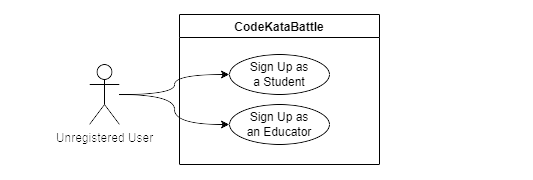
\includegraphics[width=1\linewidth]{UseCasesUU.png}
        \caption{Use Cases Diagram for Unregistered Users.} 
        \label{fig:UnregisteredUC}%
    \end{center}
\end{figure}



\begin{figure}[H]
    \begin{center}
        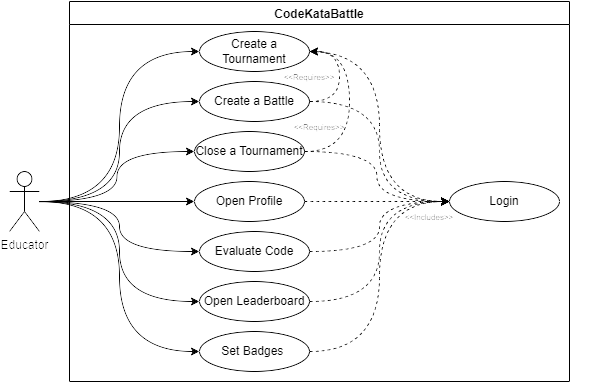
\includegraphics[width=1\linewidth]{UseCasesED.png}
        \caption{Use Cases Diagram for Educators.}
        \label{fig:EducatorUC}%
    \end{center}
\end{figure}



\begin{figure}[H]
    \begin{center}
        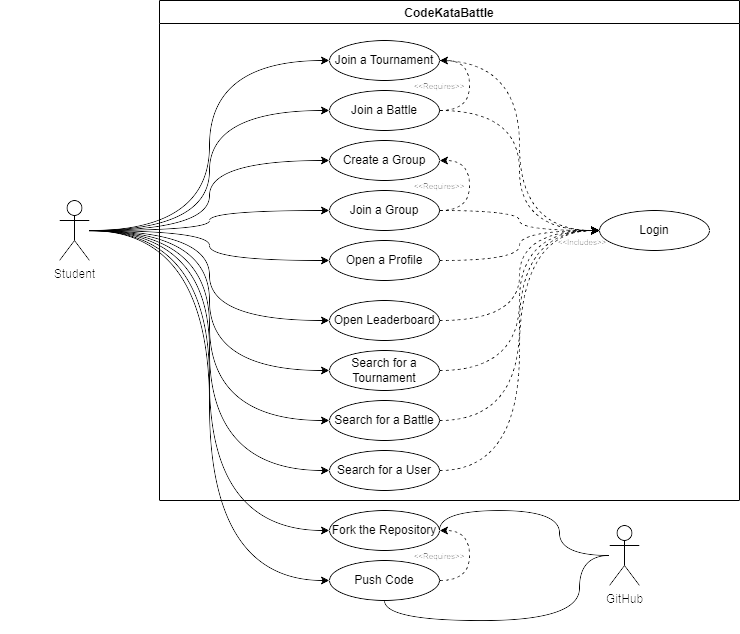
\includegraphics[width=1\linewidth]{UseCasesST.png}
        \caption{Use Cases Diagram for Students.}
        \label{fig:StudentUC}%
    \end{center}
\end{figure}

\newpage
\subsection{Use cases}
\label{subsec: use_cases}%
\newcounter{uc}
\setcounter{uc}{1}
\newcommand{\cuc}{\theuc\stepcounter{uc}}
In this section, they are explained and represented the main identified use cases.\\
There is a table with entry conditions, event flow, exit conditions and exception for each of them, and a sequence diagram that shows the messages exchanged between the entities and the called functions. \\


\subsubsection*{UC\cuc . Signup as ED}
\begin{center}
    \begin{longtable}{|l|p{0.75\linewidth}|}
        \hline
        \textbf{Actor}            & ED, eMail provider\\
        \hline
        \textbf{Entry conditions} & The ED is not already registered in CKB and has to search the CKB URL in the browser search bar \\
        \hline
        \textbf{Event Flow}       & 1 - CKB shows the login form.  \\
        & 2 - The ED clicks on “Create an Account” button.   \\
        & 3 - CKB shows the signup form.    \\
        & 4 - The ED inserts his name, surname, nickname, eMail and password in the form and also ticks on the “Signup as Educator” checkbox.  \\
        & 5 - The ED clicks on the “Register” button.  \\
        & 6 - CKB checks all the credentials.  \\
        & 7 - If credentials are correct CKB sends a confirmation eMail to the ED through the eMail provider.  \\
        & 8 - The ED clicks on the confirmation link.    \\
        \hline
        \textbf{Exit condition}   & CKB allows the ED to access to the CKB system. \\       
        \hline
        \textbf{Exceptions}       & \begin{itemize}
            \item The eMail address is already linked to an account. In this case an error message is shown and the ED is redirected to the profile creation settings.
            \item Invalid password if it is shorter than 8 characters, if it doesn’t have at least 1 number and/or 1 capital letter and/or a special character. In this case an error message is shown and the ED is redirected to the profile creation settings.
            \item  The nickname is already used. An error is shown and the ED is redirected to the profile creation settings.
        \end{itemize}\\
        \hline
        \caption{Signup as ED use case.}
        \label{tab: signup_as_ED_use_case}
    \end{longtable}
\end{center}

\begin{figure}[H]
    \begin{center}
        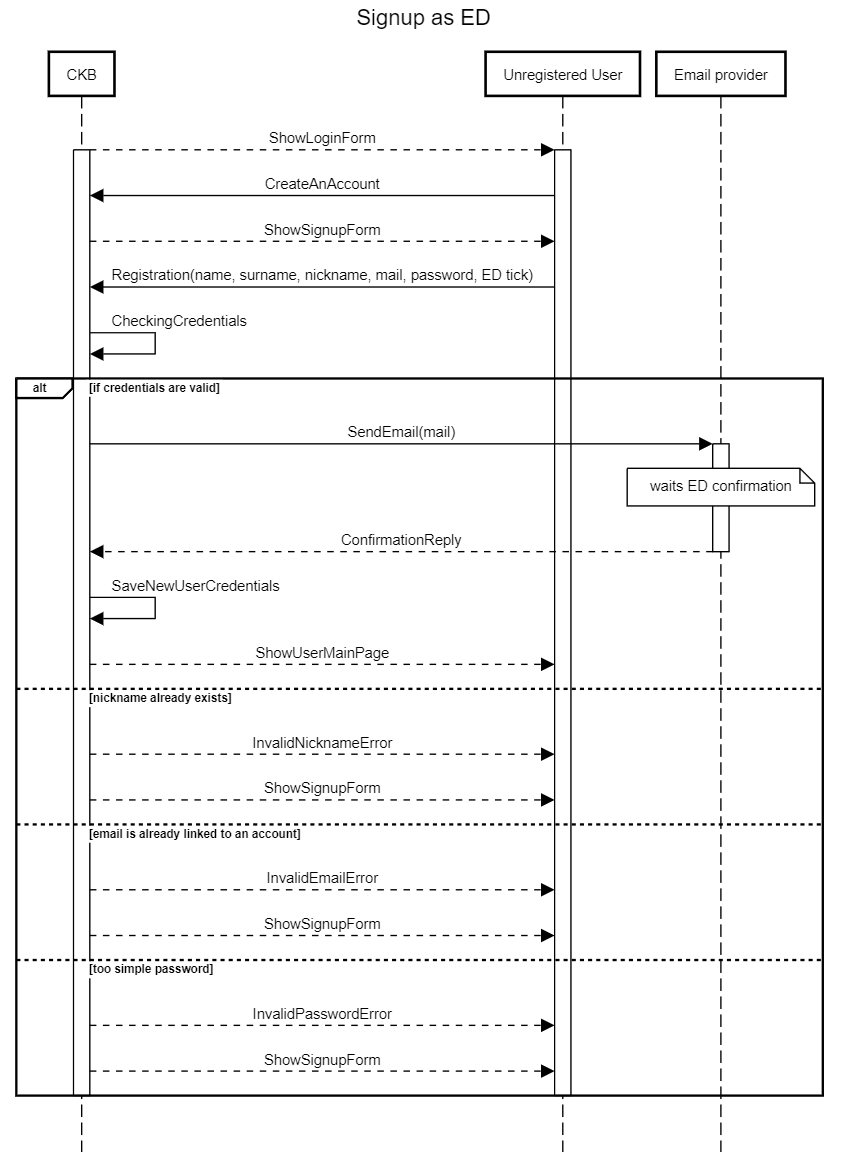
\includegraphics[width=1\linewidth]{SequenceDiagrams/Signup as ED.png}
        \caption{Signup as ED sequence diagram.}
        \label{fig:signup_as_ED_seqd}%
    \end{center}
\end{figure}

\subsubsection*{UC\cuc . Signup as ST}
\begin{center}
    \begin{longtable}{|l|p{0.75\linewidth}|}
        \hline
        \textbf{Actor}            & ST, eMail provider \\
        \hline
        \textbf{Entry conditions} & The ST is not already registered in CKB and has to search the CKB URL in the browser search bar \\
        \hline
        \textbf{Event Flow}       & 1 - CKB shows the login form.  \\
        & 2 - The ST clicks on “create an account” button.  \\
        & 3 - CKB shows the signup form.  \\
        & 4 - The ST inserts his name,surname, nickname and password in the form.  \\
        & 5 - The ST clicks on the “Register” button.  \\
        & 6 - CKB checks all the credentials.  \\
        & 7 - If credentials are correct CKB sends a confirmation eMail to the ST through an eMail provider.  \\
        & 8 - The ST clicks on the confirmation link. \\
        \hline
        \textbf{Exit condition}   & CKB allows the ST to access to the CKB system. \\
        \hline
        \textbf{Exceptions}       & \begin{itemize}
            \item The eMail address is already linked to an account. In this case an error message is shown and the ST is redirected to the profile creation settings.
            \item Invalid password if it is shorter than 8 characters, if it doesn’t have at least 1 number and/or 1 capital letter and/or a special character. In this case an error message is shown and the ST is redirected to the profile creation settings.
            \item The nickname is already used. An error is shown and the ST is redirected to the profile creation settings.
        \end{itemize} \\
        \hline
        \caption{Signup as ST use case.}
        \label{tab: signup_as_ST_use_case}
    \end{longtable}
\end{center}

\begin{figure}[H]
    \begin{center}
        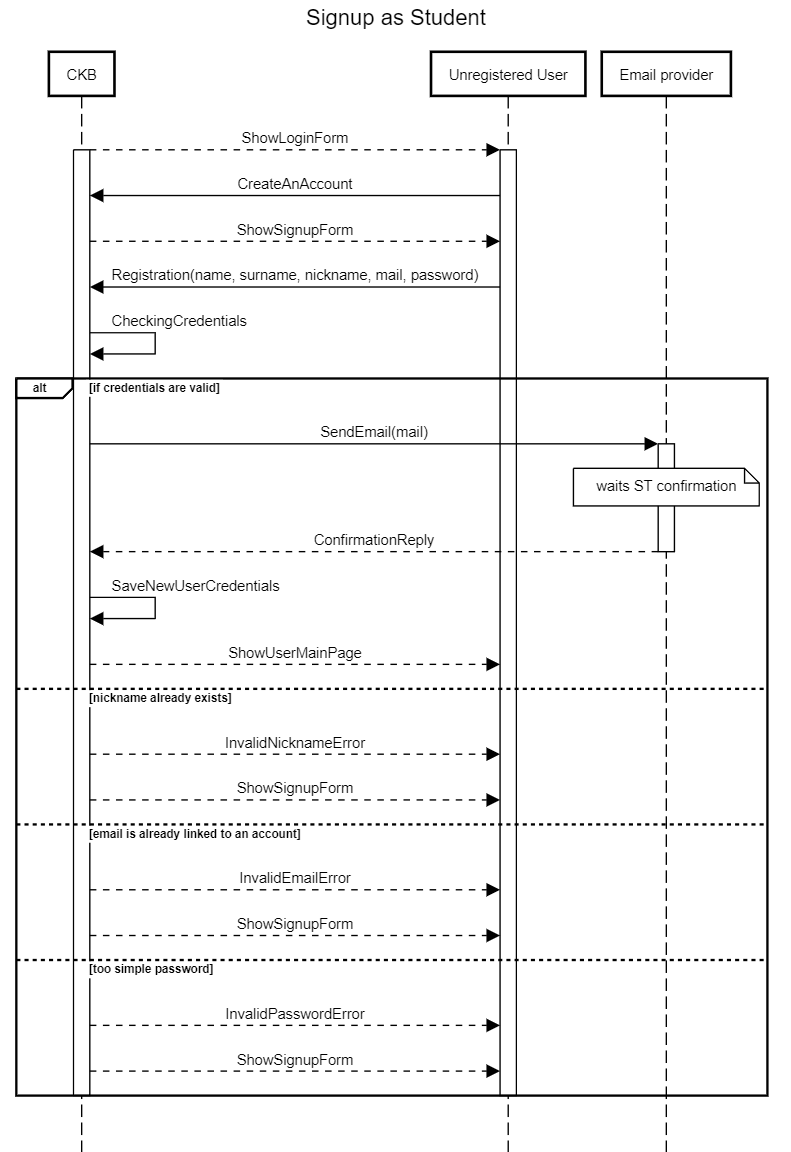
\includegraphics[width=1\linewidth]{SequenceDiagrams/Signup as ST.png}
        \caption{Signup as ST sequence diagram.}
        \label{fig:signup_as_ST_seqd}%
    \end{center}
\end{figure}

\subsubsection*{UC\cuc . Login}
\begin{center}
    \begin{longtable}{|l|p{0.75\linewidth}|}
        \hline
        \textbf{Actor}            & Users\\
        \hline
        \textbf{Entry conditions} & The User should be registered in CKB and has to search the CKB URL in the browser search bar \\
        \hline
        \textbf{Event Flow}       & 1-\ CKB shows the login form.  \\
        & 2-\ The User inserts his nickname and password in the form.\\
        & 3-\ The User clicks on the "Login" button.       \\                               
        & 4-\ CKB checks the credentials.  \\
        \hline
        \textbf{Exit condition}   & CKB allows the User to access to the CKB system. \\
        \hline
        \textbf{Exceptions}       & Incorrect eMail or password. An error message is shown and the User is redirected back to the Login page. \\
        \hline
        \caption{Login use case.}
        \label{tab: login_use_case}
    \end{longtable}
\end{center}

\begin{figure}[H]
    \begin{center}
        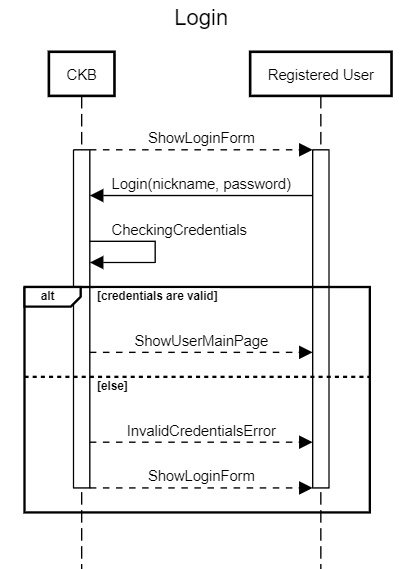
\includegraphics[width=.5\linewidth]{SequenceDiagrams/login v2.png}
        \caption{Login sequence diagram.}
        \label{fig:login_seqd}%
    \end{center}
\end{figure}

\subsubsection*{UC\cuc . Create a Tournament}
\begin{center}
    \begin{longtable}{|l|p{0.75\linewidth}|}
        \hline
        \textbf{Actor}            & ED\\
        \hline
        \textbf{Entry conditions} & The ED is correctly logged in. The ED has decided to create a Tournament. The ED is on his profile page. \\
        \hline
        \textbf{Event Flow}       & 1-\ The ED clicks on “Create a Tournament” button.       \\
        & 2-\ CKB returns the create Tournament form.   \\
        & 3-\ The ED writes the Tournament name, sets the deadline for STs to subscribe and chooses and writes the other EDs nicknames to grant them permissions to create new Battles.        \\
        & 4-\ CKB stores the data of the Tournament.        \\
        & 5-\ CKB sends a notification to the chosen EDs.        \\
        & 6-\ CKB notifies all the STs of the creation of the Tournament.        \\
        & 7-\ CKB checks if the tick on the create badge is true and if it is so CKB retrives all the ED's previously used Badges and redirects the ED to the Badges requirement page.\\
        & 8-\ If that's not the case CKB return the Tournament main page. \\
        \hline
        \textbf{Exit condition}   & The Tournament is correctly created and a confirmation message is shown to the ED.        \\
        \hline
        \textbf{Exceptions}        & \begin{itemize}
            \item The Tournament’s name is null or already exists. An error message is shown and the ED is redirected back to create Tournament settings.
            \item The EDs chosen are non-existent, or the creator chooses other ED that have already permission in this Tournament. An error message is shown to the ED and the ED is redirected to create Tournament settings.
            \item The registration deadline is a date before the day the Tournament is created. An error message is shown to the ED and a new deadline has to be chosen and the ED  is redirected to create Tournament settings.
         \end{itemize}    \\
        \hline
        \caption{Create a Tournament use case.}
        \label{tab: create_a_Tournament_use_case}
    \end{longtable}
\end{center}

\begin{figure}[H]
    \begin{center}
        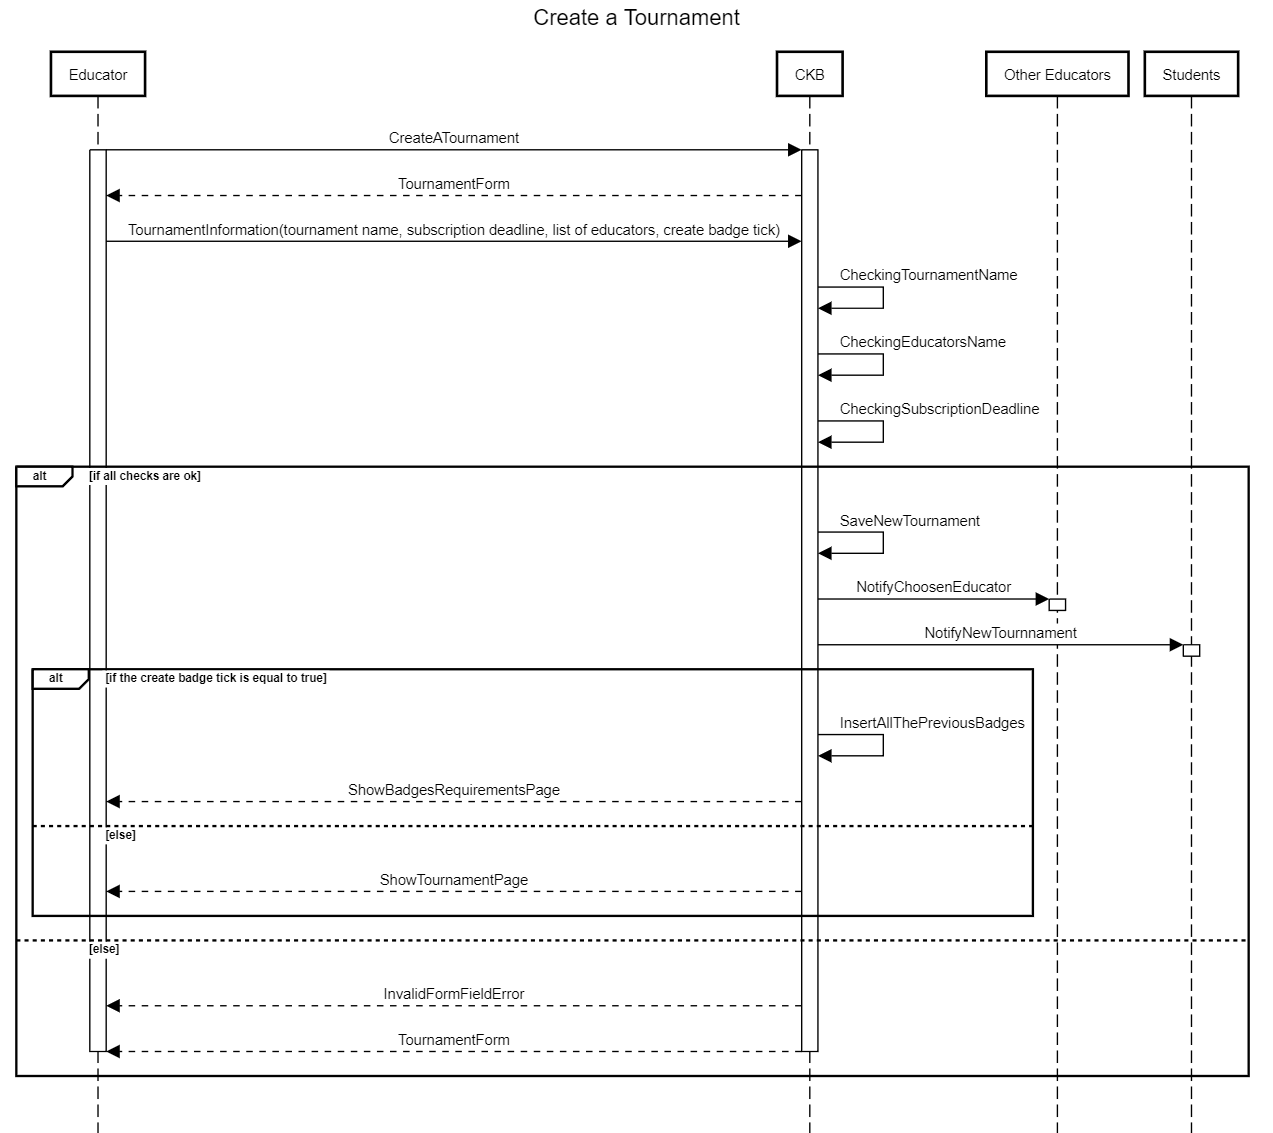
\includegraphics[width=1\linewidth]{SequenceDiagrams/Create a Tournament v2.png}
        \caption{Create a Tournament diagram.}
        \label{fig:create_a_Tournament_seqd}%
    \end{center}
\end{figure}

\newpage

\subsubsection*{UC\cuc . Join a Tournament}
\begin{center}
    \begin{longtable}{|l|p{0.75\linewidth}|}
        \hline
        \textbf{Actor}            & ST  \\
        \hline
        \textbf{Entry conditions} & The ST is correctly logged in. The ST has decided to join a Tournament.   \\
        \hline
        \textbf{Event Flow}       & 1-\ The ST search the keyword of a Tournament into the search box \\
        & 2-\ CKB returns the result from the search. \\
        & 3-\ The ST clicks on the new Tournament’s name.        \\
        & 4-\ CKB redirects the Student to the main page of the Tournament. \\
        & 5-\ The ST clicks on the “Join Tournament” button. \\
        & 6-\ CKB saves the ST as one of the competitors of the Tournament. \\
        & 7-\ CKB shows a confirm message and redirects the ST to the page that contains the current Leaderboard of the Tournament (the Tournament main page). \\
        \hline
        \textbf{Exit condition}   & The ST is now part of the Tournament and will be notified whenever a new Battle will be available.        \\
        \hline
        \textbf{Exceptions}        & \begin{itemize}
            \item Nothing is found from the research. In this case the ST will be redirectd back to the home page.
            \item The Tournament already ended. In this case is shown an error message and the ST is redirected to the final Leaderboard of the Tournament (the Tournament main page).
            \item The ST already joined the Tournament. In this case CKB will not show any error messages, but will redirect the ST to the current Leaderboard of the Tournament (the Tournament main page).
            \item The Deadline already expired. An error message is shown and the ST is redirected back to the Home Page.
        \end{itemize}    \\
        \hline
        \caption{Join a Tournament use case.}
        \label{tab: join_a_Tournament_use_case}
    \end{longtable}
\end{center}

\begin{figure}[H]
    \begin{center}
        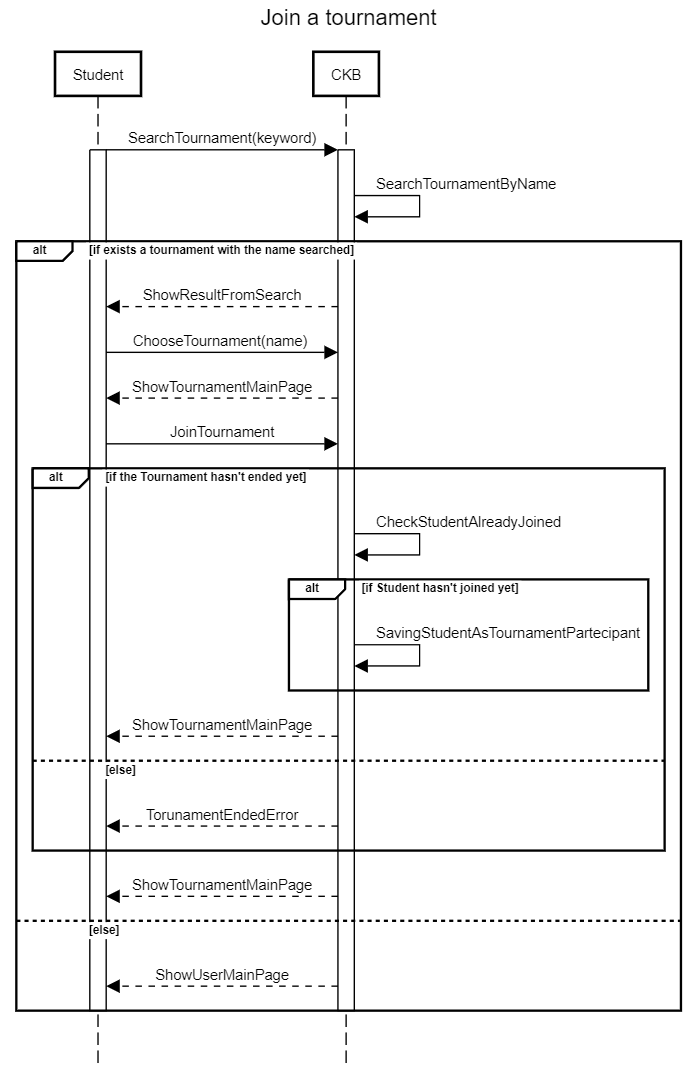
\includegraphics[width=.8\linewidth]{SequenceDiagrams/Join a tournament v2.png}
        \caption{Join a Tournament diagram.}
        \label{fig:join_a_Tournament_seqd}%
    \end{center}
\end{figure}

\newpage

\subsubsection*{UC\cuc . Create a Battle}
\begin{center}
    \begin{longtable}{|l|p{0.75\linewidth}|}
        \hline
        \textbf{Actor}            & ED \\
        \hline
        \textbf{Entry conditions} & The ED is logged in. The ED is in the Tournament page. The ED has decided to create a Battle.        \\
        \hline
        \textbf{Event Flow}       & 1-\ ED clicks on “Create new Battle” button.        \\
        & 2-\ CKB redirects ED to the create Battle form.        \\
        & 3-\ The ED uploads the code kata.        \\
        & 4-\ The ED writes the Battle name.        \\
        & 5-\ The ED sets the minimum and maximum number of STs per group.        \\
        & 6-\ The ED sets the registration deadline.      \\
        & 7-\ The ED sets the final submission deadline.      \\
        & 8-\ The ED sets additional configurations for scoring.        \\
        & 9-\ CBK checks the parameters inserted by the ED.        \\
        & 10-\ CKB create a new github repository \\
        & 11-\ CKB creates a new Battle and redirect the ED to the new Battle main page.        \\
        & 12-\ CKB sends a notification to all STs subscribed to the Tournament         \\
        \hline
        \textbf{Exit condition}   & The Battle is correctly created and the ED is redirected to the Battle main page.        \\
        \hline
        \textbf{Exceptions}        & \begin{itemize}
                \item The Battle’s name is null or already exists. An error message is shown, the ED is redirected back to the create Battle settings.
                \item The maximum number of students per group is lesser than the minimum.  An error message is shown to the ED and the ED is redirected to the create Battle settings.
                \item The minimum number of students per group is lesser or equal than zero.  An error message is shown to the ED and the ED is redirected to the create Battle.
                \item The registration deadline is a date before the day the Battle is created. An error message is shown to the ED and a new deadline has to be chosen and the ED is redirected to create Battle settings.   
                \item  The final submission deadline is a date before the registration deadline. An error message is shown to the ED and a new deadline has to be chosen and the ED is redirected to create Battle settings.  
                \item The code kata is not valid. An error message is shown to the ED and the ED is redirected to create Battle settings. 
        \end{itemize}    \\
        \hline
        \caption{Create a Battle use case.}
        \label{tab: create_a_Battle_use_case}
    \end{longtable}
\end{center}

\begin{figure}[H]
    \begin{center}
        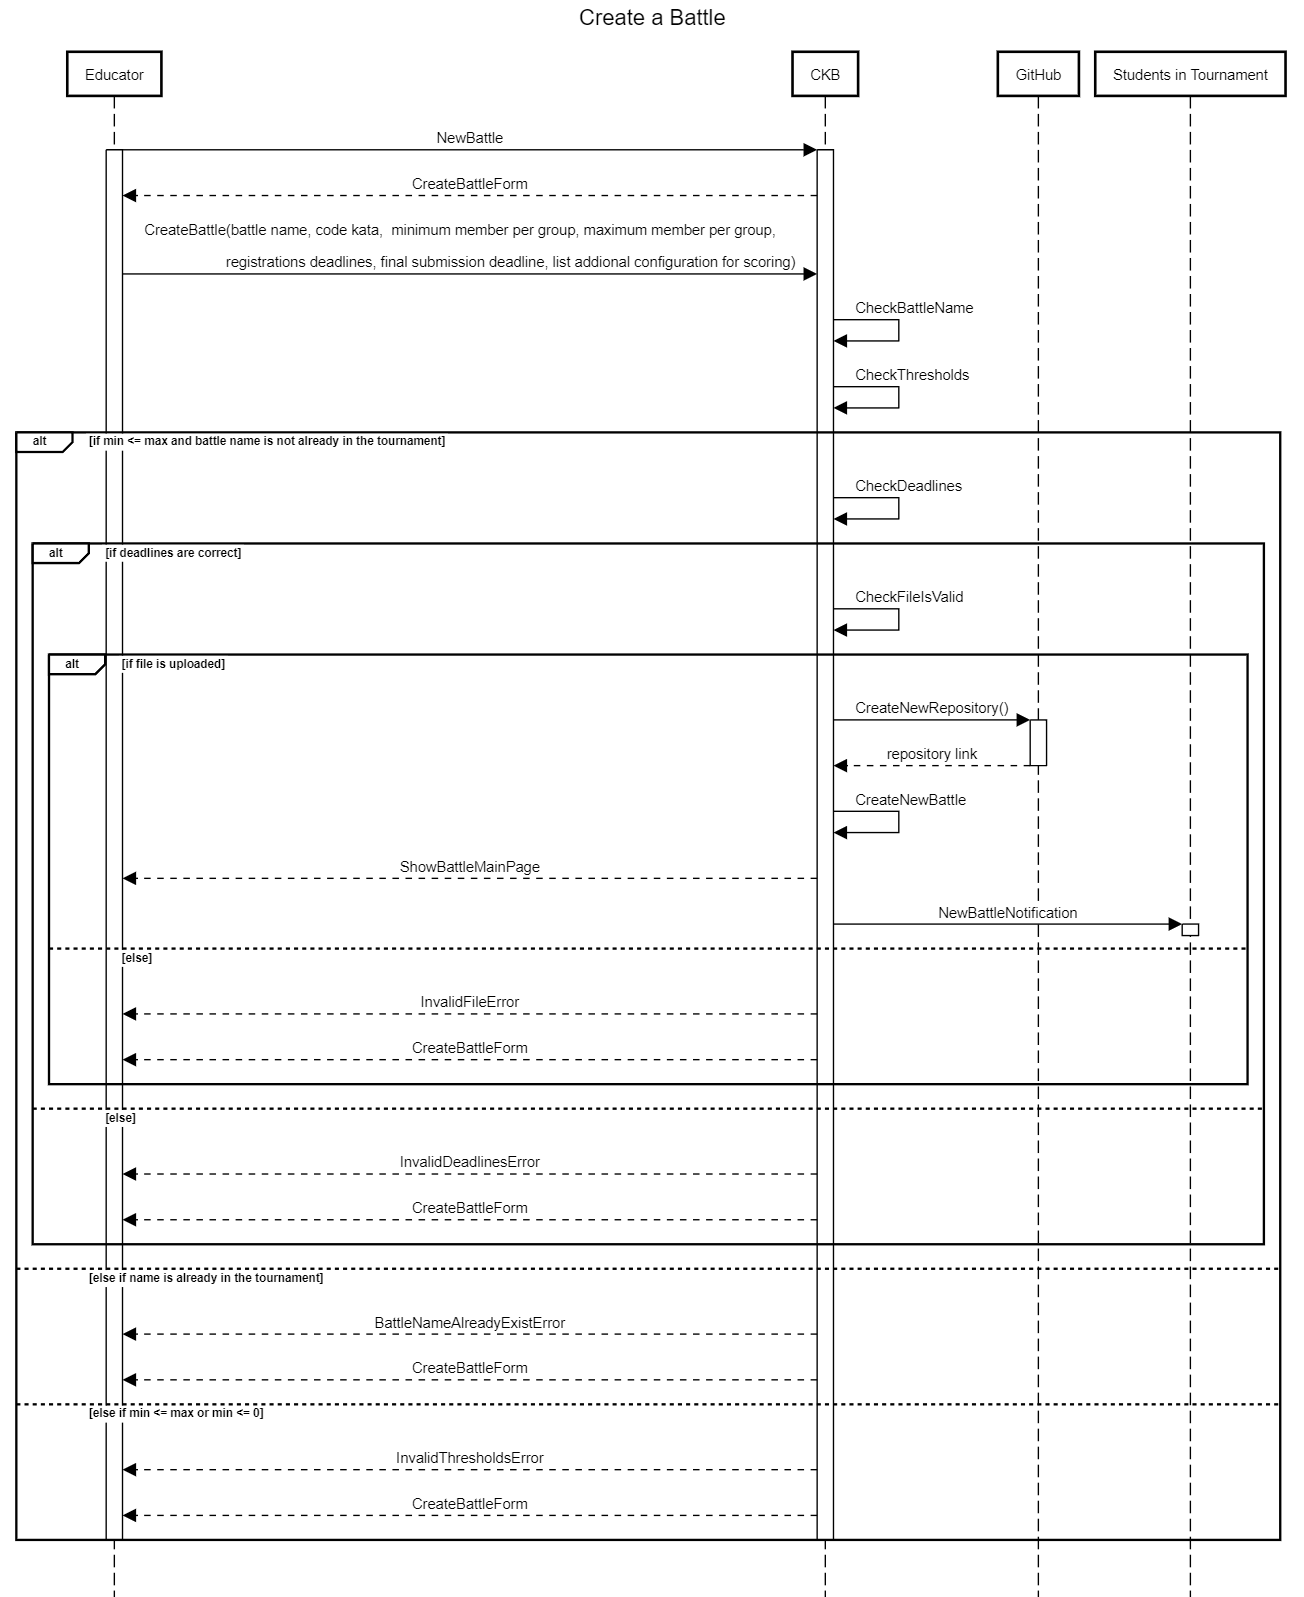
\includegraphics[width=1\linewidth]{SequenceDiagrams/Create a Battle v2.png}
        \caption{Create a Battle sequence diagram.}
        \label{fig:create_a_battle_seqd}%
    \end{center}
\end{figure}

\newpage

\subsubsection*{UC\cuc . Join a Battle}
\begin{center}
    \begin{longtable}{|l|p{0.75\linewidth}|}
        \hline
        \textbf{Actor}            & ST \\
        \hline
        \textbf{Entry conditions} & The ST is correctly logged in and it is in the Tournament main page. The ST has decided to join a Battle.        \\
        \hline
        \textbf{Event Flow}       & 1-\ The ST clicks on a tournament        \\
        & 2-\ CKB redirects the ST to the page that has the list of all the Battles of the Tournament (Tournament main page).        \\
        & 3-\ The ST clicks on the “Join Battle” button near the Battle name.        \\
        & 4-\ CKB checks that the deadline has not expired.\\
        & 5-\ CKB checks that the ST joined the Tournament that contains this Battle.   \\
        & 6-\ CKB redirects the ST to the CreateGroup page of the Battle.        \\
        \hline
        \textbf{Exit condition}   & The ST, after the subscription deadline end, will be able to create a group and then confirm the participation to the Battle        \\
        \hline
        \textbf{Exceptions}        & \begin{itemize}
            \item The ST isn’t in the Tournament that this Battle is part of. In this case CKB shows an error message, the ST is redirected back to the Tournament main page.
            \item The Battle already ended or already started. In this case  CKB shows an error message, the ST is redirected to the final Leaderboard of the Battle.
            \item The ST already joined the Battle. In this case CKB will not show any error messages, but will redirect the ST to the CreateGroup page.
         \end{itemize}    \\
        \hline
        \caption{Join a Battle use case.}
        \label{tab: join_a_Battle_use_case}
    \end{longtable}
\end{center}

\begin{figure}[H]
    \begin{center}
        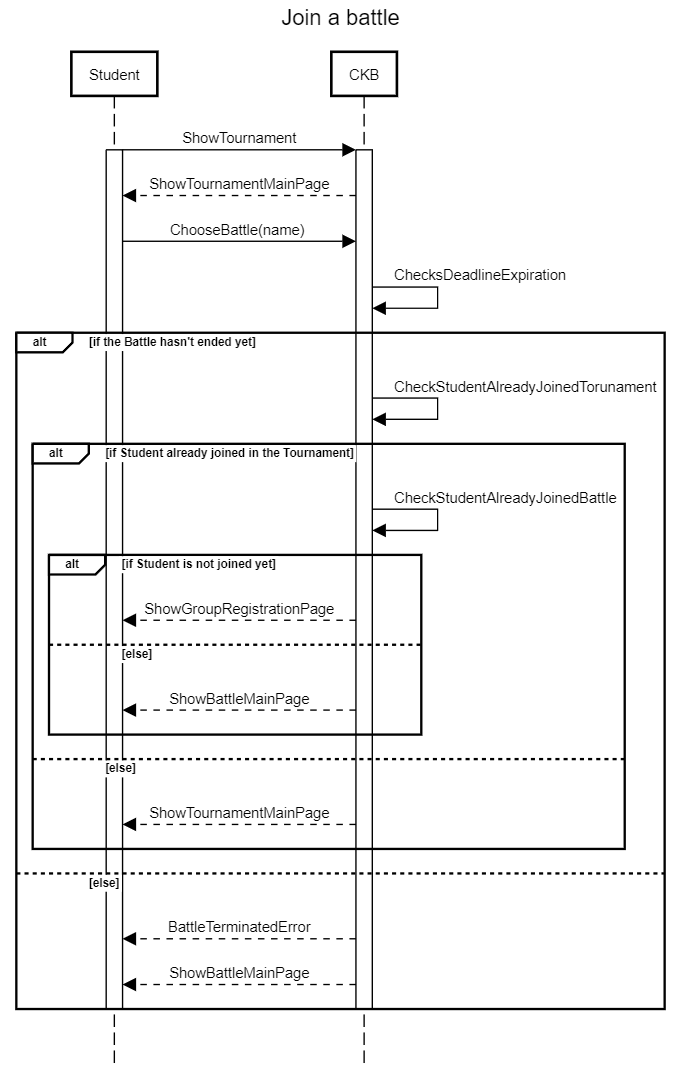
\includegraphics[width=.8\linewidth]{SequenceDiagrams/Join a battle v2.png}
        \caption{Join a battle sequence diagram.}
        \label{fig:join_a_battle_seqd}%
    \end{center}
\end{figure}

\newpage

\subsubsection*{UC\cuc . Create a group and Battle confirmation}
\begin{center}
    \begin{longtable}{|l|p{0.75\linewidth}|}
        \hline
        \textbf{Actor}            & ST   \\
        \hline
        \textbf{Entry conditions} & The ST is correctly logged in and it is in the CreateGroup page. The ST has decided to join a Battle.        \\
        \hline
        \textbf{Event Flow}       & 1-\ The ST inserts the STG name.        \\
        & 2-\ The ST inserts another ST's nickname and clicks on the “Invite” button and then.        \\
        & 3-\ CBK checks if the ST joined the competition and notifies other students of an invitation.  \\
        & 4-\ The other STs can decide to accept or reject the invitation clicking on the “Accept” or “Reject” button inside the notification.        \\
        & 5-\ CKB shows to the ST that has created the STG the different state of the various invitation requests (3 state : accepted, rejected, pending)(only the first \(n\)-invited STs that accept the invite are considered part of the group)(where \(n\) is the maximum number decided by the ED in the create Battle form).         \\
        & 6-\ The ST can click on the “Confirm Group” button.        \\
        & 7-\ CKB checks if the number of members respects the limits given by ED during the Battle creation.         \\
        & 8-\ CKB saves the ST and the STG as one of the competitors of the Battle.        \\
        & 9-\ CKB shows a confirmation message and redirects the ST to the main page of the Battle.        \\
        \hline
        \textbf{Exit condition}   & The ST is now a competitor in the Battle and he can starts committing after the creation group deadline expires        \\
        \hline
        \textbf{Exceptions}        & \begin{itemize}
            \item The STG name already exists in the Battle. In this case CKB shows an error message and the ST is redirected back to the CreateGroup page.
            \item The STG already joined the Battle. In this case CKB will not show any error messages, but will redirect the ST to the current Leaderboard of the Battle.
            \item The number of STs in the group is wrong. CKB will show an error and redirect the ST to the CreateGroup page.
            \item If the creation group deadline expires, all the STs without group or all the STG not confirmed will be kicked out from the Battle.
            \item If the invited ST has not already joined in the competition or if the nickname does not exist, CKB sends an error and redirects the ST to the CreateGroup page.
         \end{itemize}  \\
        \hline
        \caption{Create a group and Battle confirmation use case.}
        \label{tab: create_a_group_and_Battle_confirmation_use_case}
    \end{longtable}
\end{center}

\begin{figure}[H]
    \begin{center}
        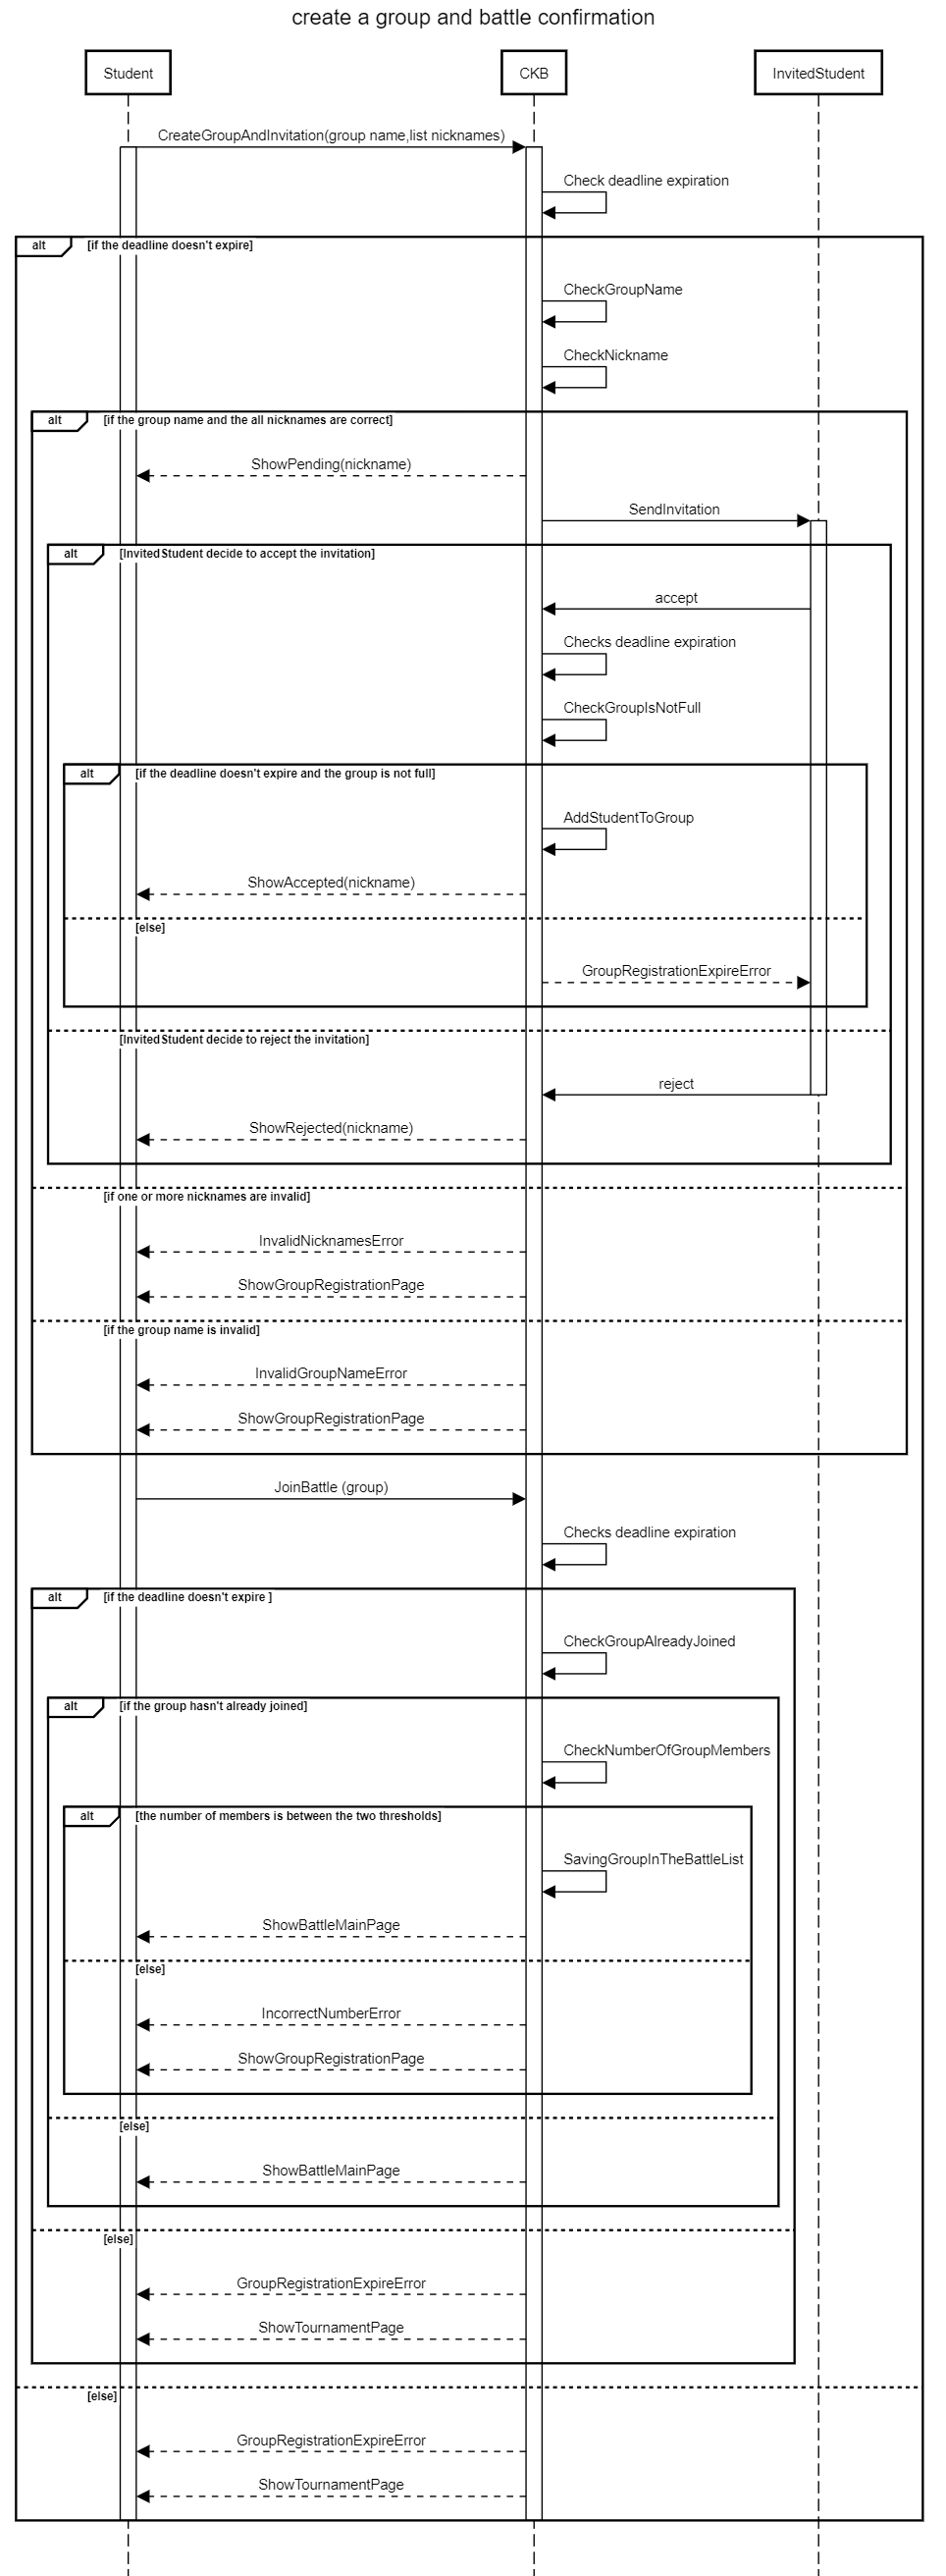
\includegraphics[width=0.5\linewidth]{SequenceDiagrams/create a group and battle confirmation.png}
        \caption{Create a group and Battle confirmation sequence diagram.}
        \label{fig:create_a_group_and_battle_confirmation_seqd}%
    \end{center}
\end{figure}

\subsubsection*{UC\cuc . Open a profile}
\begin{center}
    \begin{longtable}{|l|p{0.75\linewidth}|}
        \hline
        \textbf{Actor}            & ST or ED \\
        \hline
        \textbf{Entry conditions} & The User is logged in. The User should be in a Leaderboard (both Battle or Tournament) page for retreiving a ST profile from it or an ED profile from the owner name of the Tournament (or from the list of all the EDs)        \\
        \hline
        \textbf{Event Flow}       & 1-\ User clicks on a ST's nickname (from the Leaderboard) or ED's nickname (from the Tournament owner or from the list of all the EDs).        \\
        & 2-\ CKB returns the profile page of the selected User.        \\
        \hline
        \textbf{Exit condition}   & User is able to know particular information of the User that he had selected.        \\
        \hline
        \textbf{Exceptions}        &  The User is not found. In this case the User will be redirected back to the previous page.\\
        \hline
        \caption{Open a profile use case.}
        \label{tab: open_a_profile_use_case}
    \end{longtable}
\end{center}

\begin{figure}[H]
    \begin{center}
        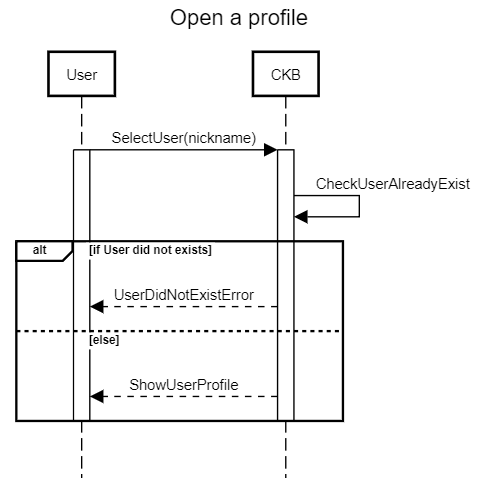
\includegraphics[width=.5\linewidth]{SequenceDiagrams/Open a profile.png}
        \caption{Open a profile sequence diagram.}
        \label{fig:open_a_profile_seqd}%
    \end{center}
\end{figure}

\newpage

\subsubsection*{UC\cuc . Search for a profile}
\begin{center}
    \begin{longtable}{|l|p{0.75\linewidth}|}
        \hline
        \textbf{Actor}            & ST or ED\\
        \hline
        \textbf{Entry conditions} & The User is logged in  \\
        \hline
        \textbf{Event Flow}       & 1-\ User clicks on the search bar.        \\
        & 2-\ User writes another User's nickname or a keyword of it. \\
        & 3-\ CKB returns the list of the Users that contain the written keyword in their nickname.         \\
        \hline
        \textbf{Exit condition}   & User is able to find the User that he was searching.        \\
        \hline
        \textbf{Exceptions}        &  None is found from the research. In this case the User will be redirectd back to the previous page.\\
        \hline
        \caption{Search for a profile use case.}
        \label{tab: search_for_a_profile_use_case}
    \end{longtable}
\end{center}

\begin{figure}[H]
    \begin{center}
        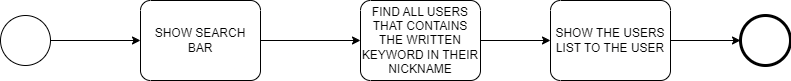
\includegraphics[width=.5\linewidth]{SequenceDiagrams/search for a profile.png}
        \caption{Search for a profile sequence diagram.}
        \label{fig:search_for_a_profile_seqd}%
    \end{center}
\end{figure}

\newpage

\subsubsection*{UC\cuc . Search for a Tournament}
\begin{center}
    \begin{longtable}{|l|p{0.75\linewidth}|}
        \hline
        \textbf{Actor}            & ST or ED  \\
        \hline
        \textbf{Entry conditions} & The User is logged in  \\
        \hline
        \textbf{Event Flow}       & 1-\ User clicks on the search bar.       \\
        & 2-\ User writes a Tournament's name or a keyword of it. \\
        & 3-\ CKB returns the list of the Tournaments that contain the written keyword in their name.         \\
        \hline
        \textbf{Exit condition}   & User is able to find the Tournament that he was searching.        \\
        \hline
        \textbf{Exceptions}        & Nothing is found from the research. In this case the User will be redirected back to the previous page.\\
        \hline
        \caption{Search for a Tournament use case.}
        \label{tab: search_for_a_Tournament_use_case}
    \end{longtable}
\end{center}

\begin{figure}[H]
    \begin{center}
        \includegraphics[width=.6\linewidth]{SequenceDiagrams/Search for a Tournament.png}
        \caption{Search for a Tournament sequence diagram.}
        \label{fig:search_for_a_Tournament_seqd}%
    \end{center}
\end{figure}

\newpage

\subsubsection*{UC\cuc . Evaluate a code}
\begin{center}
    \begin{longtable}{|l|p{0.75\linewidth}|}
        \hline
        \textbf{Actor}            & ED \\
        \hline
        \textbf{Entry conditions} & The ED is correctly logged. During the Consolidation Stage the Educator decides to check a STG’s code.        \\
        \hline
        \textbf{Event Flow}       & 1-\  The ED clicks on a battle in the Leaderboard (in Tournament main page)     \\
        & 2-\   CKB shows the Battle Main page.     \\
        & 3-\   The ED clicks the “Analyze source code” button that corresponds to a STG. \\
        & 4-\   CKB shows the source code to the ED.     \\
        & 5-\   The ED manually checks the code.     \\
        & 6-\   The ED assign a score to the STG code.     \\
        \hline
        \textbf{Exit condition}   & CKB updates the new score to the STG code       \\
        \hline
        \textbf{Exceptions}        & \begin{itemize}
            \item The Consolidation Stage already ended, an error message is shown and the ED is redirected to the battle Leaderboard page.
            \item The ED awards the STG a improper score, like a score beyond the minimum and maximum bounds decided by the ED during the Creation Phase. An error message is shown and the ED is redirected to the battle Leaderboard page.
         \end{itemize}    \\
        \hline
        \caption{Evaluate a code use case.}
        \label{tab: evaluate_a_code_use_case}
    \end{longtable}
\end{center}


\begin{figure}[H]
    \begin{center}
        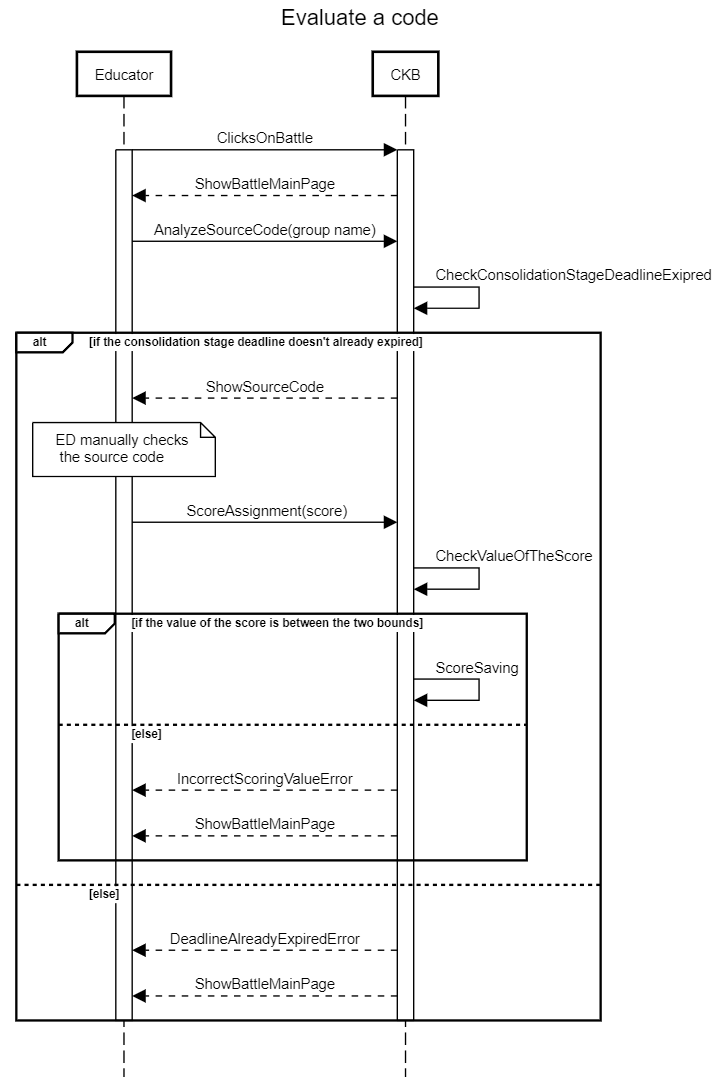
\includegraphics[width=.6\linewidth]{SequenceDiagrams/Evaluate a code v2.png}
        \caption{Evaluate a code sequence diagram.}
        \label{fig:evaluate_a_code_seqd}%
    \end{center}
\end{figure}

\newpage

\subsubsection*{UC\cuc . Create a new Badge}
\begin{center}
    \begin{longtable}{|l|p{0.75\linewidth}|}
        \hline
        \textbf{Actor}            & ED \\
        \hline
        \textbf{Entry conditions} & The ED is correctly logged. During the Torunament creation the ED has ticked the "Create Badge" setting.        \\
        \hline
        \textbf{Event Flow}      
        & 1-\ The ED inserts the Badge name, description and the rules to obtain a new Badge. \\
        & 2-\ The ED clicks on the "Create Badge" button. \\
        & 3-\ CKB checks the Badge's details. \\
        & 4-\ CKB saves the Badge's details. \\
        & 5-\ CKB return the Tournament main page. \\
        \hline
        \textbf{Exit condition}   & CKB adds the Badge to the Tournament information.      \\
        \hline
        \textbf{Exceptions}        & \begin{itemize}
            \item The Badge's name is null or already exists. An error message is shown and the ED is redirected back to the create Badge settings.
            \item The Badge's description is null. An error message is shown and the ED is redirected back to the create Badge settings.
            \item The Badge's rules are null. An error message is shown and the ED is redirected back to the create Badge settings.
         \end{itemize}    \\
        \hline
        \caption{Create a new Badge use case.}
        \label{tab: create_a_badge_use_case}
    \end{longtable}
\end{center}

\begin{figure}[H]
    \begin{center}
        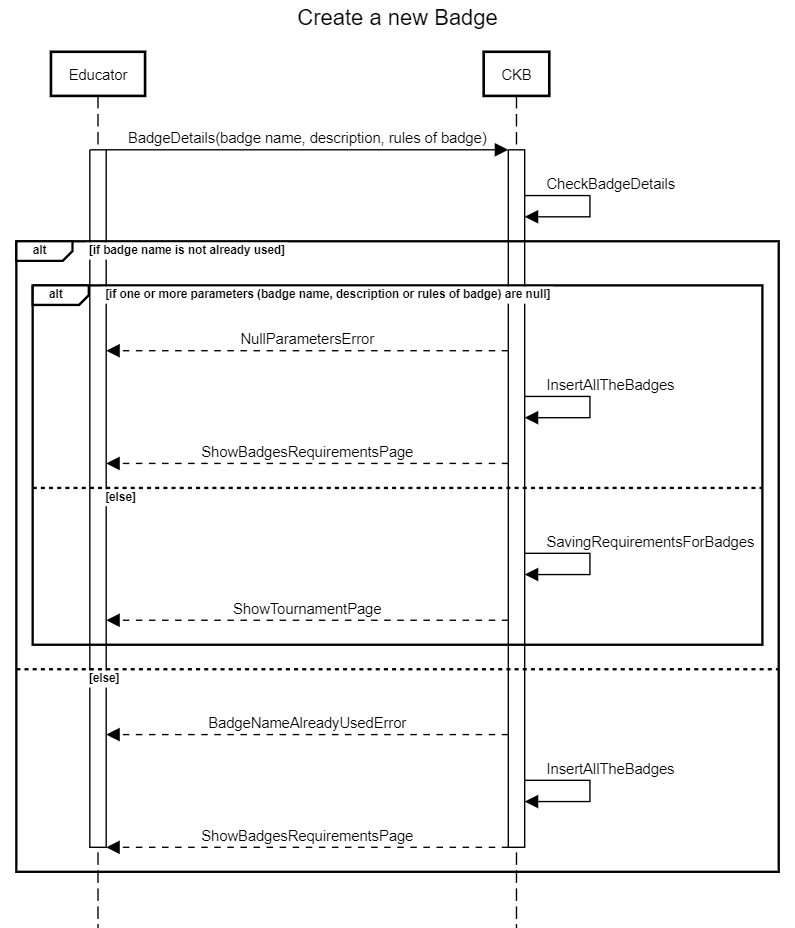
\includegraphics[width=.6\linewidth]{SequenceDiagrams/Create a new Badge.png}
        \caption{Create a new Badge sequence diagram.}
        \label{fig:create_a_new_badge_seqd}%
    \end{center}
\end{figure}

\newpage

\subsubsection*{UC\cuc . Modify an existing Badge}
\begin{center}
    \begin{longtable}{|l|p{0.75\linewidth}|}
        \hline
        \textbf{Actor}            & ED \\
        \hline
        \textbf{Entry conditions} & The ED is correctly logged. During the Torunament creation the ED has ticked the "Create Badge" setting.        \\
        \hline
        \textbf{Event Flow}       
        & 1-\ The ED clicks on a previously created Badge name. \\
        & 2-\ CKB shows to the ED the "Modify Badge" form \\
        & 3-\ The ED modifies the Badge name, description or the rules to obtain this Badge. \\
        & 4-\ The ED clicks on the "Modify Badge" button. \\
        & 5-\ CKB checks the Badge's details. \\
        & 6-\ CKB saves the Badge's details. \\
        \hline
        \textbf{Exit condition}   & CKB adds the modified Badge to the Tournament information. \\
        \hline
        \textbf{Exceptions}        & \begin{itemize}
            \item The modified Badge's name is null. An error message is shown and the ED is redirected back to the create Badge settings.
            \item The modified Badge's description is null. An error message is shown and the ED is redirected back to the create Badge settings.
            \item The modified Badge's rules are null. An error message is shown and the ED is redirected back to the create Badge settings.
            \item The modified Badge's name does not belongs to the ED.An error message is shown and the ED is redirected back to the create Badge settings.
         \end{itemize}    \\
        \hline
        \caption{ Modify an existing Badge use case.}
        \label{tab: modify_badge_use_case}
    \end{longtable}
\end{center}

\begin{figure}[H]
    \begin{center}
        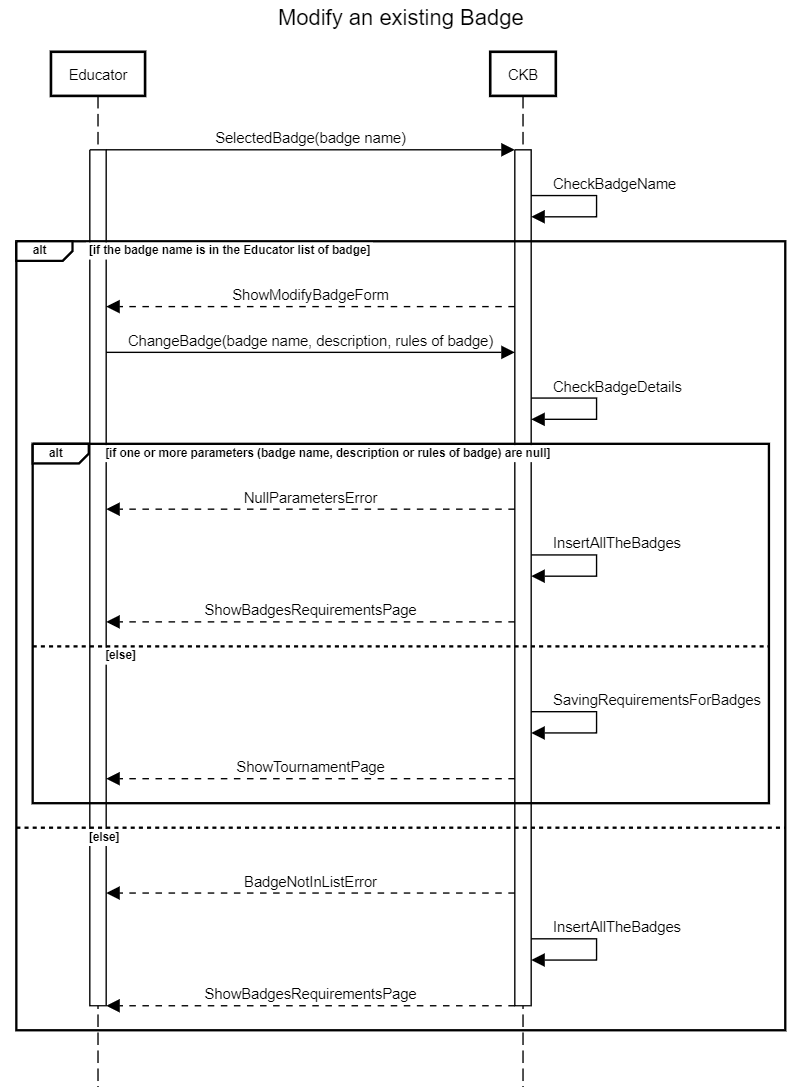
\includegraphics[width=.6\linewidth]{SequenceDiagrams/Modify an existing Badge.png}
        \caption{Modify an existing Badge sequence diagram.}
        \label{fig:modify_an_existing_badge_seqd}%
    \end{center}
\end{figure}

\newpage

\subsection{Mapping on goals}
\label{subsec:mapping_on_goals}%
\textbf{G1 - Allow an ED to create a Tournament.}
\begin{itemize}
    \item R1: CKB allows unregistered Users to sign up.
    \item R2: CKB allows registered EDs to login.
    \item R4: CKB allows EDs to create Tournaments.
    \item R5: CKB allows EDs to grant the permissions of a Tournament to other EDs.
    \item R15: CKB allows EDs to choose which Badges to award in a certain Tournament.
    \item R17: CKB allows EDs to close a Tournament.
    \item R27: CKB sends notifications to every ST when a new Tournament is created.
    \item R50: CKB sends notifications to the ED when he receives the permission to create Battles in a Tournament.
\end{itemize}

\vspace{1.5cm}
\textbf{G2 - Allow a ST to subscribe to a specific Tournament before the registration deadline.}
\begin{itemize}
    \item R1: CKB allows unregistered Users to sign up.
    \item R3: CKB allows registered STs to login.
    \item R20: CKB allows STs to join a Tournament.
    \item R39: CKB allows STs to check the list of ongoing Tournaments.
    \item R43: CKB sends notification to every ST involved in a Tournament when the Tournament is closed and the final ranks are available.
    \item R46: CKB shall communicate with the mailing system in order to allow Users to register their account.
\end{itemize}


\vspace{1.5cm}
\textbf{G3 - Allow an ED to create a Battle.}
\begin{itemize}
    \item R6: CKB allows EDs to create Battles.
    \item R7: CKB allows EDs to uploads the code kata of a Battle.
    \item R8: CKB allows EDs to set the minimum and the maximum number of STs per group of a Battle.
    \item R9: CKB allows EDs to set a registration deadline of a Battle.
    \item R10: CKB allows EDs to set a submission deadline of a Battle.
    \item R11: CKB allows EDs to set additional configuration for the scoring system of a Battle.
    \item R12: CKB allows EDs to set functional aspects for the scoring system of a Battle.
    \item R16: CKB allows EDs to assign a score manually during the consolidation stage.
    \item R28: CKB sends notifications when a new Battle is created to every ST which is participating in the Tournament that the Battle is part of.
    \item R30: CKB creates a GH repository of the code kata when the registration deadline for the Battle expires.
    \item R31: CKB sends the link of the GH repository to every STG that participates in the Battle.
    \item R32: CKB evaluates the STG's work every time a push is made on GH and calculates Battle score for the STG.
    \item R33: CKB updates the Battle Leaderboard once a new score is registered.
    \item R46: CKB shall communicate with the mailing system in order to allow Users to register their account.
\end{itemize}


\vspace{1.5cm}
\textbf{G4 - Allow any User to visualize the profile of other Users and their Badges.}
\begin{itemize}
    \item R18: CKB allows EDs to visualize the profile of another User.
    \item R19: CKB allows STs to visualize the profile of another User.
    \item R25: CKB stores the information about the Users.
    \item R26: CKB shall ensure security of data. 
\end{itemize}


\vspace{1.5cm}
\textbf{G5 - Allow a ST to subscribe to a specific Battle before the registration deadline.}
\begin{itemize}
    \item R21: CKB allows STs to join a Battle.
    \item R22: CKB allows STs to create a new STG.
    \item R23: CKB allows STs to join a STG.
    \item R24: CKB allows STs to invite other STs in their STG.
    \item R29: CKB sends notifications to a ST when he receives an invitation to be part of STG.
    \item R31: CKB sends the link of the GH repository to every STG that participates in the Battle.
\end{itemize}


\vspace{1.5cm}
\textbf{G6 - Allow STs to submit their code before the submission deadline.}
\begin{itemize}
    \item R16: CKB allows EDs to assign a score manually during the consolidation stage.
    \item R32: CKB evaluates the STG's work every time a push is made on GH and calculates Battle score for the STG.
    \item R33: CKB updates the Battle Leaderboard once a new score is registered.
    \item R34: CKB updates the Tournament Leaderboard once a new score is registered.
    \item R37: CKB allows EDs to analyze the code of a STG.
    \item R38: CKB sends notification to every ST involved in a Tournament when the Tournament is closed and the final ranks are available.
    \item R44: CKB shall communicate with the GH API in order to calculate a new score every time a push action is made by a STG.
    \item R45: CKB shall communicate with the external tool in order to calculate the score of a STG.
    \item R47: STs need to fork the GH repository of the Battle they are participating in.
    \item R48: STs need to push their code in the GH repository in order to have their code evaluated.
\end{itemize}


\vspace{1.5cm}
\textbf{G7 - Allow an ED to set Badges for deserving STs.}
\begin{itemize}
    \item R13: CKB allows EDs to create new Badges.
    \item R14: CKB allows EDs to choose the rules related to the awarding of Badges.
    \item R15: CKB allows EDs to choose which Badges to award in a certain Tournament.
    \item R49: CKB shall assign the Badges to all STs that fulfill their requirements.
\end{itemize}


\vspace{1.5cm}
\textbf{G8 - Allow any User to view the result and the progress of a Tournament.}
\begin{itemize}
    \item R34: CKB updates the Tournament Leaderboard once a new score is registered.
    \item R40: CKB allows EDs to check the list of ongoing Tournaments.
    \item R41: CKB allows STs to check the Leaderboard of a Tournaments.
    \item R42: CKB allows EDs to check the Leaderboard of a Tournaments.
    \item R43: CKB sends notification to every ST involved in a Tournament when the Tournament is closed and the final ranks are available.
\end{itemize}


\vspace{1.5cm}
\textbf{G9 - Allow any User to view the results of a Battle.}
\begin{itemize}
    \item R33: CKB updates the Battle Leaderboard once a new score is registered.
    \item R35: CKB allows STs to check the Leaderboard of a Battle.
    \item R36: CKB allows EDs to check the Leaderboard of a Battle.
\end{itemize}

\vspace{1.5cm}
\newcounter{rtt}
\setcounter{rtt}{1}
\newcommand{\crt} {\thertt\stepcounter{rtt}}
\begin{center}
     \begin{longtable}{|l|c|c|c|c|c|c|c|c|c|}
    \hline
    \textbf{Requirements} & \textbf{G1} & \textbf{G2} & \textbf{G3} & \textbf{G4} & \textbf{G5} & \textbf{G6} & \textbf{G7} & \textbf{G8} & \textbf{G9}\\ \hline
    R\crt & \checkmark & \checkmark &  &  &  &  &  &  &  \\ \hline
    R\crt & \checkmark &  &  &  &  &  &  &  &  \\ \hline
    R\crt &  & \checkmark &  &  &  &  &  &  &  \\ \hline
    R\crt & \checkmark &  &  &  &  &  &  &  &  \\ \hline
    R\crt & \checkmark &  &  &  &  &  &  &  &  \\ \hline
    R\crt &  &  & \checkmark &  &  &  &  &  &  \\ \hline
    R\crt &  &  & \checkmark &  &  &  &  &  &  \\ \hline
    R\crt &  &  & \checkmark &  &  &  &  &  &  \\ \hline
    R\crt &  &  & \checkmark &  &  &  &  &  &  \\ \hline
    R\crt &  &  & \checkmark &  &  &  &  &  &  \\ \hline
    R\crt &  &  & \checkmark &  &  &  &  &  &  \\ \hline
    R\crt &  &  & \checkmark &  &  &  &  &  &  \\ \hline
    R\crt &  &  &  &  &  &  & \checkmark &  &  \\ \hline
    R\crt &  &  &  &  &  &  & \checkmark &  &  \\ \hline
    R\crt &\checkmark  &  &  &  &  &  & \checkmark &  &  \\ \hline
    R\crt &  &  & \checkmark &  &  & \checkmark &  &  &  \\ \hline
    R\crt &\checkmark  &  &  &  &  &  &  &  &  \\ \hline
    R\crt &  &  &  & \checkmark &  &  &  &  &  \\ \hline
    R\crt &  &  &  & \checkmark &  &  &  &  &  \\ \hline
    R\crt &  & \checkmark &  &  &  &  &  &  &  \\ \hline
    R\crt &  &  &  &  & \checkmark &  &  &  &  \\ \hline
    R\crt &  &  &  &  & \checkmark &  &  &  &  \\ \hline
    R\crt &  &  &  &  & \checkmark &  &  &  &  \\ \hline
    R\crt &  &  &  &  & \checkmark &  &  &  &  \\ \hline
    R\crt &  &  &  & \checkmark &  &  &  &  &  \\ \hline
    R\crt &  &  &  & \checkmark &  &  &  &  &  \\ \hline
    R\crt & \checkmark &  &  &  &  &  &  &  &  \\ \hline
    R\crt &  &  & \checkmark &  &  &  &  &  &  \\ \hline
    R\crt &  &  &  &  & \checkmark &  &  &  &  \\ \hline
    R\crt &  &  & \checkmark &  &  &  &  &  &  \\ \hline
    R\crt &  &  & \checkmark &  & \checkmark &  &  &  &  \\ \hline
    R\crt &  &  & \checkmark &  &  & \checkmark &  &  &  \\ \hline
    R\crt &  &  & \checkmark &  &  & \checkmark &  &  & \checkmark \\ \hline
    R\crt &  &  &  &  &  & \checkmark &  & \checkmark &  \\ \hline
    R\crt &  &  &  &  &  &  &  &  & \checkmark \\ \hline
    R\crt &  &  &  &  &  &  &  &  & \checkmark \\ \hline
    R\crt &  &  &  &  &  & \checkmark &  &  &  \\ \hline
    R\crt &  &  &  &  &  & \checkmark &  &  &  \\ \hline
    R\crt &  & \checkmark &  &  &  &  &  &  &  \\ \hline
    R\crt &  &  &  &  &  &  &  & \checkmark &  \\ \hline
    R\crt &  &  &  &  &  &  &  & \checkmark &  \\ \hline
    R\crt &  &  &  &  &  &  &  & \checkmark &  \\ \hline
    R\crt &  &  \checkmark&  &  &  &  &  & \checkmark &  \\ \hline
    R\crt &  &  &  &  &  & \checkmark &  &  &  \\ \hline
    R\crt &  &  &  &  &  & \checkmark &  &  &  \\ \hline
    R\crt &  &  \checkmark& \checkmark &  &  &  &  &  &  \\ \hline
    R\crt &  &  &  &  &  & \checkmark &  &  &  \\ \hline
    R\crt &  &  &  &  &  & \checkmark &  &  &  \\ \hline
    R\crt &  &  &  &  &  &  & \checkmark &  &  \\ \hline
    R\crt & \checkmark &  &  &  &  &  &  &  &   \\ \hline
\caption{Traceability Matrix for Goals and Requirements}
\label{tab:traceability}
\end{longtable}
\end{center}


\section{Performance requirements}
\label{sec:performance_requirements}%
\paragraph{Number of concurrent Users:} According to recent researches, websites with a similar goal of CKB, has about 1.8 million Users. We want our website to attract at least 25\% of those Users, which means CKB should be able to handle up to 500,000 Users simultaneously. This is important for making sure our website works well for a good number of people, giving them a smooth and enjoyable experience.
\paragraph{Data storage:} CKB needs to save and manage all the details about both STs and EDs. Additionally, it has to store information about all the Tournaments, including the associated Battles. When a Tournament is closed all the data about it won’t be canceled and a reference of it and of the Battles remains in the ED’s page .
\paragraph{Time response:} Every operation that is directly executed by CKB, i.e. register, login, create, join and evaluate, should be in the domain of milliseconds. Other operations such as the ones that involve GH, the mailing system and the External Tools cannot be guaranteed by CKB itself.


\newpage
\section{Design constraints}
\label{sec:design_constraints}%


\subsection{Standard compliance}
\label{subsec:standard compliance}%%
The system must be compliant to the EU's GDPR (General Data Protection Regulation), a set of regulations that is designed in order to protect the personal data, the privacy and security of the EU's citizens. 


\subsection{Hardware limitations}
\label{subsec:hardware_limitations}%
The only hardware limitations are the support for a reliable internet connection and for a Web Browser.


\section{Software system attributes}
\label{sec:software_system_attributes}%

\subsection{Reliability}
\label{subsec:reliability}%
The system has to be fault tolerant in order to prevent the propagation of errors and to guarantee a continuous usability of the system.

\subsection{Availability}
\label{subsec:availability}%
The system must be available the most time possible, with a minimum value of 99.9\% (three-nines) of time. In this way the system will be unavailable for only 8.76 hours a year. \\
It shall be prevented a case scenario in which a maintenance break occurs near to Battle's end, therefore there must be as few maintenance breaks as possible, with them possibly at nightime.

\subsection{Security}
\label{subsec:security}%
The system must control the access rights of the Users. The system shall grant both authentication, verifying the identity of the Users that attempt to login and authorization, verifying the permission of the already logged Users to perform certain requested actions. \\
Measures to protect the database will be adopted, such as defense against query injections, and password and Users' personal data stored will be encrypted.


\subsection{Maintainability}
\label{subsec:maintainability}%
The system must be designed using scalable and reusable models in order to permit future addition of features with minimum effort. \\
Ordinary maintenance has to be scheduled at nightime, in order to keep the services available when the User traffic is high.

\subsection{Portability}
\label{subsec:portability}%
The system must be accessible by the Users from every kind of Web Browser.\\ 
There are no particular portability requirements server side.



